\documentclass[a4paper,oneside]{report}

\usepackage{amsmath}
\usepackage{amssymb}
\usepackage{caption}
\usepackage[english]{babel}
\usepackage{fancyhdr} 
\usepackage{float}
\usepackage{multirow}
\usepackage[pdftex]{graphicx}
\usepackage{listings}      
\usepackage{pdfpages}
\usepackage{setspace}
\usepackage{url}
\usepackage{wrapfig}

\lstset{language=Ada,
numberstyle=\footnotesize,
%basicstyle=\ttfamily\footnotesize,
basicstyle=\footnotesize,
numbers=left,
stepnumber=1,
frame= lines,
breaklines=true}

\makeatletter


%
% Some custom definitions
%

% add horizontal lines
\newcommand{\HRule}{\rule{\linewidth}{0.5mm}}
\newcommand{\HRuleLight}{\rule{\linewidth}{0.1mm}}

% custom part page
\def\part#1#2
{
	\par\break
  	\addcontentsline{toc}{part}{#1}
	\noindent
	\null	
	\HRuleLight\\[0.0cm]
	\vspace{20pt}	 
	\begin{flushright} 		
  	{\Huge \bfseries \noindent #1}\\
  	\vspace{30pt} 
	\begin{minipage}{0.85\textwidth}
		\begin{flushright}
		{\large \noindent #2}
		\end{flushright}
	\end{minipage}\\[0.75cm] 
	\end{flushright} 		
	\thispagestyle{empty}
	\break
}

% chapter header
\renewcommand{\@makechapterhead}[1]
{\vspace*{50\p@}{
	\parindent \z@ \raggedright \normalfont
	%\huge \bfseries \thechapter. #1
	\huge \bfseries #1
	\vspace{20pt}}}

\setcounter{secnumdepth}{-1} 
\onehalfspace
\oddsidemargin 1in 
\oddsidemargin 0.6in 
\topmargin -0.3in
\setlength{\textwidth}{14cm}
\setlength{\textheight}{23cm}
\lstset{language=C} 

\begin{document}

%
% Cover page
%
\begin{titlepage}
\begin{center}

\HRuleLight\\[0.5cm]

\Huge Programming, Concurrency and Client-Server Computing

\HRuleLight\\[0.2cm]

\large School of Computing, Engineering and Mathematics\\ \textbf{University of Brighton}

\vfill
\huge Revision Booklet\\
\large May, 2012\\

\end{center}
\end{titlepage}


%
% Table of contents
%
{
	\renewcommand\thepage{}
	\setcounter{tocdepth}{3}
	\tableofcontents
	\clearpage
}

% reset page count
\setcounter{page}{1}


%
% Start of content
%

%\section{What Makes a Good Program}
%\section{History(?)}
\chapter{Programming Languages}
\section{A comparison between Java, Ada, Haskell and Prolog}


\chapter{Concurrency}
	\section{What it is}
	
	Concurrency allows you to effectively utilise available processing power by allowing a computer to perform several different tasks simultaneously (e.g web web server requests, spell-checking whilst typing)
	
    	\subsection{Types of concurrency}
    	
    	\paragraph{Coroutines} With co-operative schedules (or coroutines), processes suspend voluntarily  when they need to wait for an event. Processes may also suspend at regular intervals during lengthy processing.
    	
    	\paragraph{Timeslicing} With pre-emptive scheduling (or timeslicing), processes are suspended as a result of interrupts from external hardware. This can present problems with shared resource access, as it is impossible to predict at what point a process will be suspended.
    	
  	\section{How it's implemented}
  	
    	\subsection{Java}
      		
      		\paragraph{Threads} Java's \emph{Thread} class can be used to implement concurrency. Each instance of the class represents a different `thread' of execution, allowing multiple processes to execute simultaneously.\\ 
\textbf{Useful methods:} \emph{Thread.start()}, \emph{Thread.run()} - thread halts on exit from run, \emph{Thread.sleep(time)}, \emph{Thread.interrupt()}, \emph{Thread.get/setPriority()}

      		\paragraph{Synchronisation} Problems will occur if two threads try to modify/access shared data simultaneously (or rather if one tries to access while one tries to modify, or both try to modify). Using a \emph{synchronized} block prevents data corruption, as only one thread is able to execute it at a time. Each Java object has an internal ‘lock’ and a queue for waiting threads; if the lock is clear, lock the object and enter the block, if the lock is set, wait. On exit from the block, clear the lock and wake up a waiting thread (if there are any). This isn't very OO, as data is only protected where it is accessed, not where it is defined. The solution is to `synchronize' an entire method.
      		
    	\subsection{Ada}
    	
      		\subsubsection{Tasks}
      		Tasks are Ada's equivalent of Java's threads; each separate task representing a separate `thread' of execution. Tasks can communicate with each other via `entry' calls. Entry points are declared in the task spec
– a task declares ‘entries’ (like procedures) in the task spec in the form of ‘accept’ statements. An entry call causes a ‘rendezvous’ between the called task and its caller. The caller waits for the task to accept the call – the accept statement waits for a call (see Listing).
         
\begin{lstlisting}[label=some-code,caption=Ada's Accept Statement] 
loop 
	select
		accept Show (Message : in String) do
			Put_Line(Message);
		end Show; or
		accept Stop;
        exit;
	end select;
end loop;
\end{lstlisting}
      		
      		Entries require a client/server relationship, as they only communicate between one task and another. This is inefficient when just accessing shared data (tasks must be rescheduled to actually pass the data).
      		
      		\subsubsection{Protected records}
      		Protected records (added in Ada 95) use shared data much more efficiently. Protected records contain private data which is accessed by public functions, entries and procedures.\\
      		
      		\noindent\textbf{Functions} are given read-only access to the data and can be executed by multiple tasks simultaneously.\\
      		
      		\noindent\textbf{Procedures} have read and write access to the data, but can only be executed by a single task at any one time. Additionally, no other tasks can be executing any other functions, procedures or entries while a procedure is executing.\\
      		
      		\noindent\textbf{Entries} are similar to procedures, but also has a guard condition which suspends the caller until it evaluates to true. 
      		
    	\subsection{Haskell}
    	
  	\section{Issues Associated With Concurrency}
  	
  	Although concurrency adds the power to do new things, it also brings with it new types of errors.
  	
    	\subsection{Deadlock}
    	Deadlock occurs when two (or more) processes require access to an inaccessible certain resource in order to continue. This usually occurs when one process has a lock on some resource which is needed by another process, which itself has a lock on a resource which the first process holds. Neither process are   able to relinquish their lock on the problem resources, as they cannot get a lock on the new resources etc. etc.\\
    	
    	\noindent All four of the following conditions are necessary for deadlock to occur: 
    	\begin{enumerate}
    		\item Tasks need to use a non-shareable resource\\ 
    			  \emph{Can be prevented by virtualising resources (e.g. print spooling on disk: printer is non-shareable, disk is shareable), though this is not always possible (e.g. a railway track is not shareable between two trains and cannot be virtualised).}
    		\item Tasks hold onto resources while waiting for extra ones\\
    			  \emph{Insist that all resources are allocated at once (task cannot proceed until all resources have been granted). This is inefficient as resources will be allocated when not needed.}
    		\item Resources cannot be taken away from tasks by a third party\\
    			  \emph{See above solution.}
    		\item There is a circular chain of tasks requesting a resource held by another task\\
    			  \emph{Resources can be prioritised, allocated in priority order. A process must finish using (and release) high priority resources before it can use a lower priority one.}
    	\end{enumerate}
    	
    	It is not always possible to recover from deadlock. The operating system may check for deadlocks by checking the thread table for circularities. If a deadlock is detected, the OS will kill one of the locked processes until the deadlock is broken. This can obviously have severe implications for the program. Similarly, if deadlocks are not dealt with within the program, it may become unresponsive, forcing the user to kill the program manually.
    	
    	\subsection{Livelock}
    	Livelock is similar to deadlock, except that tasks are still able to proceed. However, execution is useless in that tasks will not be able to make any meaningful progress. For example, ethernet, where collisions cause back-offs of exponentially increasing length (this variation in wait time will normally eventually break the lock). Where contention is low, probability of livelock is low enough to ignore (although this is not a suitable response in safety-critical situations). Livelock isn't as easily definable as deadlock, the system may appear to be functioning. Deadlocked threads cannot be scheduled, whereas livelocked ones can. If a `fair' scheduling algorithm is used, livelock can be avoided (e.g. if a guarantee is made that every request is eventually dealt with). 
    	
    	\subsection{Starvation}
    	Starvation occurs if one or more tasks are `starved' of resources by other tasks. This might result from a poor choice of task priorities so that high priority tasks will hog resources that lower priority tasks also need, meaning that the lower priority tasks are never able to function. Even if the high-priority thread is blocked, the low-priority thread still can’t get hold of the resource it needs.
    	
    	\subsection{Priority inversion}
    	This occurs if a high-priority task (A) is unable to access a resource which is held by a lower-priority task (B). If A suspends until the resource is free, B is able to proceed. This means that a low-priority process is taking precedence over a high-priority process. If thread A waits in a loop for the resource, the result is a perpetual livelock: B never runs because A is running, but A is always waiting for B.
    	
    	\subsection{The Dining Philosophers}
    	\begin{quotation}\emph{
    	Five philosophers go to a Chinese restaurant and are seated round a circular table.  There is a single chopstick between each pair of philosophers. Each philosopher alternately thinks (which involves putting down any chopsticks that the philosopher is holding) and eats (which involves picking up two chopsticks - only one chopstick can be picked up at a time).}
    	\end{quotation}
    	
    	The dining philosophers is an example of a problem which exhibits the main dangers associated with concurrent systems. \textbf{Deadlock:} Each philosopher picks up left chopstick and waits forever for the right chopstick to reappear. \textbf{Livelock:} Same as above, but put down left chopstick if right one is unavailable. \textbf{Starvation:} Two philosophers can starve another sitting between them if they are never thinking at the same time\\
    	
\textbf{Solving the problem:} Deadlock can be avoided by providing one extra chopstick or one fewer chair, having one left-handed philosopher, allowing philosophers to snatch chopsticks from each other, philosophers put chopstick down if the other isn’t available, or allowing chopsticks to be shared.   
    	 
 	 	Livelock only requires circular waiting for unshareable resources, so can be avoided by picking up left chopstick and put it down again if chopstick not available, or snatching chopstick from neighbours.
    	 
Another solution could be to provide a bottle of soy sauce, whereby philosophers can only pick up chopsticks if they have the bottle, sauce is put down sauce after both chopsticks are collected. The bottle ensures mutual exclusion for the critical act of picking up a chopstick.
    	
\chapter{Distributed Systems}

	\section{Multi-processors}
	
	Becoming increasingly common due to their decreasing cost. Adding extra processors (or cores) is a much more cost-effective way of increasing performance. 
	
	Many embedded real-time systems are ad-hoc distributed systems, configuration determined by overall structure of system being controlled (e.g. aircraft: cockpit systems, fuel systems, wings, tailplane). Processors must be located where they are needed and networked together.
	
    	\paragraph{Tightly coupled}	Multiple processors sharing a single memory (e.g. SMP, quad Pentium motherboards). Tightly coupled systems are good for performance (i.e. more processors = faster), but bad for fault tolerance, as the system relies on shared resources. Tightly coupled systems require simpler coordination of tasks, as have shared memory (using some form of semaphore system).
    	
    	\paragraph{Loosely coupled} Distributed networks with no shared memory (e.g. Beowulf), with nodes (processors) communicating over a Local Area Network. This makes coordination more difficult (as there's no shared memory), but also means that fault tolerance is possible by introducing duplicate nodes. An issue which is introduced with loosely-coupled systems is that of whether to use homogenous (with identical processors) or heterogenous (different processors) systems. Homogenous processors are able to compare results at regular intervals, using a `majority' voting process allows any failing nodes to be identified. However, if the voting is done through a central unit, failures in that unit will fail the whole system. This can be solved using a distributed analog voting mechanism whereby each unit generates an analog signal (e.g. a voltage) which is applied to one or more common carriers. The resultant voltage indicates result. Introducing heterogenous systems can introduce extra communication difficulties based on the systems' architecture (e.g. using big endian vs. little endian). Fault tolerance is also more difficult, as processor speeds will likely vary, development costs are much higher, and truly independent development is difficult to achieve.
    	
    	\paragraph{Example Use-case: The (Now Defunct) Space Shuttle} 
    	Uses four main processors in a homogenous system, and uses majority voting. If one processor fails, it leaves three others while it is being replaced, the remaining three can continue majority voting. Also has one heterogenous backup processor which is used in emergencies when two of the four main processors have failed (kept as a warm standby, monitoring the main processors to keep up to date).
    	
   	\subsection{Problems}
   	
   	Loosely coupled systems have most issues with reliability. One reason being that there's no common timebase; each processor's view of the system may be inconsistent. This can be solved by delaying message passing.\\
   	
   	\textbf{Failure modes}: transient, permanent, intermittent; fail safe (known state), fail soft (‘graceful degradation’); fail uncontrolled, fail late (correct values but too late), fail silent (no values), fail stop (no values, failure visible to other nodes)
   	\emph{Uncontrolled intermittent failures are the hardest to deal with, as parts of the system will act `traitorously'}

\paragraph{Issues to be addressed:}
\begin{itemize}
	\item Ensuring a consistent timebase so that all processors can tell what order events occur in.
	\item Ensuring shared resources are not accessed by multiple processors at the same time (distributed mutual exclusion).
	\item Need to be able to recognise situations where one processor deadlocks another (distributed deadlock detection).

\end{itemize}
   	
The basic problem is that distributed systems are nondeterministic (i.e. the outcome can be unpredictable due to timing issues). There are two types of nondeterminism: angelic (an ‘angel’/external agent ensures that the best choice is always made), and demonic (no assumption can be made about the choice the ‘demon’ will make). Angelic determinism is generally impossible to achieve, were it possible, any NP-complete problem could be solved in polynomial time by always selecting the ‘correct’ path to follow. The alternative is to add mechanisms to make things deterministic.   	
 		\subsection{Global state}
    	\subsection{Network issues}
    	\subsection{Mutual exclusion}
    	\subsection{Deadlock}
  	\subsection{How is it implemented}
    	\subsection{Java}
      		\subsubsection{RMI}
      		\subsubsection{CORBA}
      		\subsubsection{Jini}
      		
      		
\chapter{Networking}

	\section{Internet fundamentals}
 	
    	\subsection{TCP/IP}
    	Loosely referred to as `internet protocols', TCP/IP consists of 5 main layers: hardware, data link (e.g. device driver for Ethernet card), internet (IP), transport (TCP or UDP), application (HTTP etc.). This layered model assumes reliable data transfer at each level; each layer has its own error detection and recovery mechanisms (e.g. by requesting re-transmissions). TCP assumes that reliability is an end-to-end problem: individual packets can be lost or corrupted, and rather than each node passing the message from one endpoint to another, only the transport layer deals with errors detection and recovery. TCP assumes that hosts participate in network issues (routing, error handling, network control). Each destination layer receives the object sent by the same source layer (data link layer receives frames sent by the source data link layer etc.).
    	
    	\begin{figure}[h!]
    	    \begin{center}
    		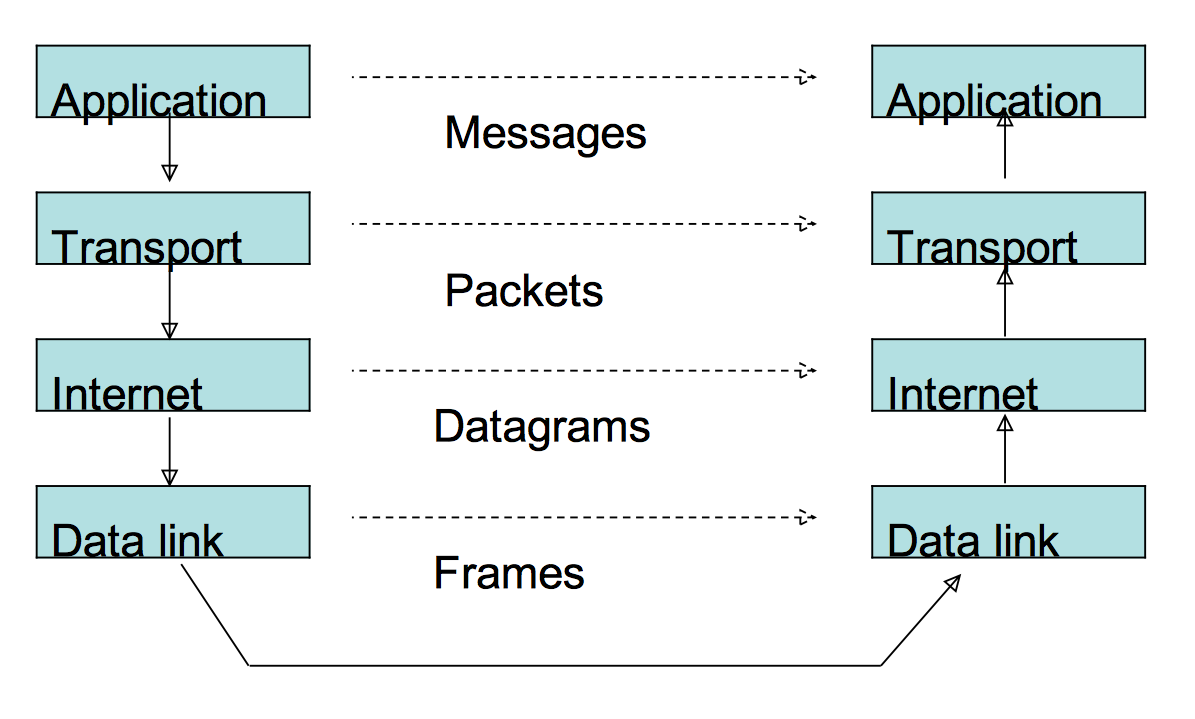
\includegraphics[width=100mm]{layering.png}
    		\caption{The TCP/IP Layered Structure}
    		\end{center}
    	\end{figure}
    	
    	\subsection{Ethernet}
    	Ethernet is a broadcast medium which has become the standard for local area networks. Ethernet stations communicate by sending each other data packets (individual blocks of data). Each Ethernet station is given a 48-bit MAC address to identify it on the network. With ethernet, every frame sent is received by every system connected to the Ethernet (including the transmitter).\\
    	
\noindent\textbf{Frame format:}
preamble - alternating 0s and 1s for synchronisation (8 octets), destination (6 octets), source (6 octets), frame type (2 octets), data (64-1500 octets), CRC (4 octets)
    	    	
\ \\ \textbf{Carrier Sense Multiple Access with Collision Detection (CSMA/CD):} Used to regulate access: A node waiting to transmits monitors the carrier signal waiting for the line to become idle, at which point it starts transmitting. If another node starts transmitting at the same time, the frame is garbled (detectable by the senders). When a collision is detected, each transmitting node ‘backs off’ for a random period. This randomness reduces chance of another collision (in the case of further collisions, the maximum period for back-off is doubled - exponential). As the network load increases, collisions become more frequent, causing more nodes to back off. This causes the network to slow down, but should not fail completely.
    	
    	\subsection{Internet Addresses}
    	Addresses are IPv4 (or 32-bit), consisting of 4 octets expressed as n.n.n.n (e.g. 127.0.0.1). The next-gen IPv6 (128-bit) consists of 6 octets (giving $\sim$1038 unique addresses).

• Address divided into network and machine number:
– subnet mask specifies how it is divided
    	
    	\subsection{ICMP}
    	\subsection{RARP}
    	\subsection{BOOTP}
    	\subsection{DHCP}
    	\subsection{Transport layer}
    	\subsection{Name resolution/DNS}

  	\section{How is it implemented}
  	
    	\subsection{Java}
    	
      		\subsubsection{Client/server}
      		Many concurrent systems are implemented as client/server systems, where a server provides a service, and clients communicate with the server to use the service (e.g. web servers and web browsers, time servers providing synchronised time). Java comes with the \emph{java.net} package which contains many network-related classes.
      		
      		\subsubsection{TCP/IP}
      		The Transmission Control Protocol over Internet Protocol allows you to connect to a specific `port' on a remote machine, and read/write data to the port (like writing to a file). TCP is similar to a phone conversation: you connect, communicate and disconnect.     		
        	\subsubsection{Sockets}
        	A socket connects to a server, and Input/OutputStreams are used to read and write the data.
        	
        	\subsubsection{Socket servers}
        	Socket servers bind to a particular port and wait for someone to connect, at which point it communicates with the client. Server sockets can be set to timeout (\emph{setSoTimeout(5000);}) so that they don't wait indefinitely for a connection.
        	
      		\subsubsection{UDP (Sockets, Packets)}
      		The User Datagram Protocol doesn't carry the same guarantee for communication: a message isn't guaranteed to reach its destination. Data is sent as an individual `packet', rather than a continuous stream of data. Having sent a request, a response may be sent (or not). As there isn't necessarily a response, the socket should be set to timeout. UDP is more efficient than TCP, and allows for data to be `multicasted' to multiple recipients. Multicasting allows broadcasting to recipients whose individual addresses aren't necessarily known. UDP is particularly relevant in video streaming for example, where it doesn't matter if odd packets (or frames) are lost.
    	
\chapter{Real-time}
  	\section{What is a real-time system}
  	
  	All computer systems model some aspect of the outside world, although the timescale doesn't necessarily match that of the real world. Real time systems are required to conform to timescales imposed by the outside world: they must work as `fast' (or `slowly') as the outside world.
  	
  	\paragraph{Hard real time}: very tight deadlines; failure to meet deadlines is catastrophic (e.g. aerospace autopilot).
  	
  	\paragraph{Soft real time}: deadlines are more flexible; failure to meet deadlines is not necessarily catastrophic (e.g. multimedia video display applications, financial payroll systems).
  
  	
  	\section{Embedded systems}
  	Real time systems are often computer systems which are part of (embedded in) a larger system
– e.g. process control, autopilot, manufacturing
• ‘Embedded’ often used as a synonym for real time
  	
  	\section{Characteristics}
  	
  	\begin{itemize}
  		\item Needs to cope with a variety of external events (where software is becoming frequently large and complex)
		\item Reliable and safe: able to detect and recover from failures
		\item Need to interact with external hardware
  		\item Need to be able to specify timing requirements (when to perform actions, when to complete actions by, what to do when deadlines are missed, importance of granularity (e.g. IBM PC clock granularity is 55ms = 100yds at 600mph)
  		\item Event-driven rather than process-driven (external events must be dealt with as they occur; event ordering is not generally predictable)
		\item Generally uses concurrent processes (each event source can be handled by a separate process)  
  		\item Must have predictable response times (factors to consider: caching/pipelining affect program speed, worst case is an order of magnitude slower than the average, fast programs \& external time)
  		\item Code must be safe (i.e. nothing `bad' will happen) and live (i.e. something `good' will eventually happen). `Eventually' must be able to be upper-bounded, as livelock can particularly be an issue in real-time systems.
  	\end{itemize}
  	
\chapter{Security}
  	\section{Password protection}
	\section{Encryption}
    	\subsection{Public-key}
    	\subsection{Steganography}
    	\subsection{SSL}
  	\section{Types of attack}
    	\subsection{Trojan}
    	\subsection{Virus}
    	\subsection{Worm}
    	\subsection{Denial of service}
    	\subsection{Mail bombing}
    	\subsection{Phishing}
    	\subsection{Keylogging}
  	\section{Protection}

\end{document}
